% Theory deck of Day 5. Skeleton: see LaTeX/templates/README.md.
% Build: bash build.sh --file Day05_Theory.tex

\documentclass[10pt]{beamer}

% Course preamble for "AI on Edge Devices" (KAUST Academy).
%
% Load this file in the main file of every new deck:
%
%   \documentclass[10pt]{beamer}
%   % Course preamble for "AI on Edge Devices" (KAUST Academy).
%
% Load this file in the main file of every new deck:
%
%   \documentclass[10pt]{beamer}
%   % Course preamble for "AI on Edge Devices" (KAUST Academy).
%
% Load this file in the main file of every new deck:
%
%   \documentclass[10pt]{beamer}
%   \input{preamble/course}
%
% Do not load preamble/packages.tex or preamble/commands.tex. Those two files
% are the older preamble of the template. No deck uses them, and they report
% LaTeX errors.
%
% This file gives these commands:
%
%   \source{...}       small source line at the bottom of the frame
%   \sourcehere{...}   small source line at the current position
%   \code{...}         inline code
%   \cmark, \xmark     check mark and cross mark, for comparison tables
%   \keypoint{...}     box for the main point of a frame
%   \exerciseframe{title}{body}   one exercise frame
%   \answerframe{title}{body}     the answer frame of that exercise
%   \theorypart{title}{exercise}  start of one part of a theory deck
%   exerciseblock                 environment: the exercise box alone
%   answerblock                   environment: the answer box alone
%   L{width}                      table column: paragraph, ragged right
%   \coursecredits                source list of the credits frame
%
% Listing styles for code: python, cpp, shell. Example:
%
%   \begin{frame}[fragile]{Read the sensor}
%     \begin{lstlisting}[style=python]
%   print("hello")
%     \end{lstlisting}
%   \end{frame}
%
% A frame that contains a listing needs the option [fragile]. A listing also
% cannot stand in the argument of a command. So write such a frame in full and
% use the environment exerciseblock in place of \exerciseframe.
%
% sections/credits.tex prints the credits frame.
%
% Check this preamble after a change:
%   bash tools/build_deck.sh Preamble_Test.tex

% ---------------------------------------------------------------- packages ---
\usepackage[utf8]{inputenc}
\usepackage{amssymb}
\usepackage{amsmath}
\usepackage{graphicx}
\usepackage{caption}
\usepackage{subcaption}
\usepackage{array}
\usepackage{booktabs}
\usepackage{multicol}
\usepackage{multirow}
\usepackage{pifont}
\usepackage{tcolorbox}
\usepackage{listings}
\usepackage{tikz}
\usetikzlibrary{arrows.meta,positioning,fit,calc,shapes.geometric}

% The theme, the logo, and the colours of the template.
\input{preamble/beamer_settings}

% ------------------------------------------------------------ frame layout ---
% Captions on a slide carry no number.
\setbeamertemplate{caption}{\insertcaption}
\setbeamerfont{caption}{size=\footnotesize}
\hypersetup{colorlinks=true,linkcolor=cardinalred,urlcolor=darkcyan}

% The cover frame (sections/cover.tex) has room for a title of one line. A
% longer title moves the date into the footer. This hook counts the lines of
% the title and moves the cover up by the height of each extra line.
\newcount\covertitlelines
\newlength{\covertitleskip}
\addtobeamertemplate{title page}{%
  \setbox0=\vbox{%
    \hsize=\dimexpr\textwidth-16pt\relax
    \usebeamerfont{title}\centering\inserttitle\par
    \global\covertitlelines=\prevgraf
    \global\covertitleskip=\baselineskip}%
  \ifnum\covertitlelines>1
    \vskip-\dimexpr\covertitleskip*\numexpr\covertitlelines-1\relax\relax
  \fi
}{}

% Table column L{width}: a paragraph column with a ragged right margin. A
% plain p{width} column justifies the text and breaks words in a narrow
% column.
\newcolumntype{L}[1]{>{\raggedright\arraybackslash}p{#1}}

% ------------------------------------------------------------ code listings ---
% beamercolorthemestanford.sty gives cardinalred, coolgray, treegreen,
% darkcyan, boxgray, and footergray.
\definecolor{codebg}{RGB}{246,245,243}

\lstdefinestyle{coursebase}{
  basicstyle=\ttfamily\scriptsize,
  keywordstyle=\color{cardinalred}\bfseries,
  commentstyle=\color{coolgray}\itshape,
  stringstyle=\color{darkcyan},
  numberstyle=\ttfamily\tiny\color{coolgray},
  backgroundcolor=\color{codebg},
  frame=single,
  rulecolor=\color{footergray},
  framesep=3pt,
  xleftmargin=2pt,
  xrightmargin=2pt,
  aboveskip=0.6em,
  belowskip=0.4em,
  showstringspaces=false,
  breaklines=true,
  breakatwhitespace=true,
  columns=fullflexible,
  keepspaces=true,
  upquote=true,
  tabsize=2,
}

\lstdefinestyle{python}{
  style=coursebase,
  language=Python,
  morekeywords={as,with,assert,None,True,False,self,async,await},
}

\lstdefinestyle{cpp}{
  style=coursebase,
  language=C++,
  morekeywords={int8_t,uint8_t,int16_t,uint16_t,int32_t,uint32_t,size_t,
                constexpr,nullptr,alignas,PROGMEM},
}

\lstdefinestyle{shell}{
  style=coursebase,
  language=sh,
  morekeywords={python3,pip,pip3,arduino-cli,mpremote,esptool.py,ollama,
                mosquitto_pub,mosquitto_sub,ffmpeg,systemctl,raspi-config},
}

% Plain \begin{lstlisting} uses the base style.
\lstset{style=coursebase}

% ---------------------------------------------------------------- commands ---
% Inline code.
\newcommand{\code}[1]{\texttt{\small #1}}

% Check mark and cross mark.
\newcommand{\cmark}{{\color{treegreen}\ding{51}}}
\newcommand{\xmark}{{\color{cardinalred}\ding{55}}}

% Source line for a figure, a table, or text from a source.
% \sourcehere prints the line at the current position, for example under a
% figure in one column. \source pushes the line to the bottom of the frame.
\newcommand{\sourcehere}[1]{{\par\scriptsize\color{coolgray}Source: #1\par}}
\newcommand{\source}[1]{\vfill\sourcehere{#1}}

% The main point of a frame.
\newcommand{\keypoint}[1]{%
  \begin{tcolorbox}[colframe=cardinalred,colback=boxgray,boxrule=0.6pt,
      arc=2pt,left=4pt,right=4pt,top=3pt,bottom=3pt]
    \textbf{Key point:} #1
  \end{tcolorbox}%
}

% ------------------------------------------------------ exercise and answer ---
% \exerciseframe and \answerframe make the complete frame. They read the body
% as a macro argument, so the body must contain no listing.
% The environments exerciseblock and answerblock hold the content alone. Use
% them inside a frame with the option [fragile] when the body has a listing.
\newtcolorbox{exerciseblock}{colframe=darkcyan,colback=boxgray,boxrule=0.8pt,
  arc=2pt,left=5pt,right=5pt,top=4pt,bottom=4pt}

\newtcolorbox{answerblock}{colframe=treegreen,colback=boxgray,boxrule=0.8pt,
  arc=2pt,left=5pt,right=5pt,top=4pt,bottom=4pt}

\newcommand{\exerciseframe}[2]{%
  \begin{frame}{Exercise: #1}
    \begin{exerciseblock}#2\end{exerciseblock}
  \end{frame}%
}

\newcommand{\answerframe}[2]{%
  \begin{frame}{Answer: #1}
    \begin{answerblock}#2\end{answerblock}
  \end{frame}%
}

% ------------------------------------------------------------ theory parts ---
% A theory deck has three parts. Each part file starts with
%   \theorypart{TITLE}{EXERCISE}
% The command starts a section of the deck. The contents frame
% (sections/dayNN/toc.tex) lists the title and the exercise of each part.
% Before part 2 and before part 3 the contents frame comes again, with the
% current part highlighted. Part 1 has no such frame, because the contents
% frame of the deck stands immediately before it.
\DeclareRobustCommand{\partexercise}[1]{\\{\footnotesize Exercise: #1}}
\newcommand{\theorypart}[2]{%
  \section[#1]{#1\texorpdfstring{\partexercise{#2}}{}}}

\setbeamertemplate{section in toc}{%
  \makebox[3.8em][l]{\textbf{Part \inserttocsectionnumber}}%
  \parbox[t]{\dimexpr\linewidth-3.8em\relax}{\raggedright\inserttocsection}}
\setbeamertemplate{section in toc shaded}[default][45]

\AtBeginSection{%
  \ifnum\value{section}>1
    \begin{frame}{Contents}
      \tableofcontents[currentsection]
    \end{frame}
  \fi}

% ----------------------------------------------------------------- credits ---
% One command for each source. Section 10 of the syllabus gives this text.
\newcommand{\creditmlsys}{\item \emph{Machine Learning Systems} by Vijay
  Janapa Reddi and contributors, Harvard University. mlsysbook.ai,
  CC BY-NC-SA 4.0.}
\newcommand{\creditraspi}{\item \emph{Edge AI Engineering: Raspberry Pi} by
  Marcelo Rovai. github.com/Mjrovai/EdgeML\_Made\_Ease\_ebook and
  github.com/Mjrovai/EdgeML-with-Raspberry-Pi, GPL-3.0.}
\newcommand{\creditxiao}{\item \emph{TinyML Made Easy: XIAO ESP32S3} by
  Marcelo Rovai. github.com/Mjrovai/XIAO-ESP32S3-Sense, Apache-2.0.}
\newcommand{\creditbigpower}{\item \emph{XIAO: Big Power, Small Board} by Lei
  Feng and Marcelo Rovai.
  github.com/Mjrovai/XIAO\_Big\_Power\_Small\_Board-ebook, GPL-3.0.}
\newcommand{\credittinymlx}{\item \emph{HarvardX TinyML courseware} by the
  TinyMLx team. github.com/tinyMLx/courseware, CC BY-NC-SA 4.0.}
\newcommand{\credittflm}{\item \emph{TensorFlow Lite Micro Arduino examples}
  by The TensorFlow Authors.
  github.com/tensorflow/tflite-micro-arduino-examples, Apache-2.0.}

% The source list of the credits frame. The default names the main textbook
% and the three companion books. A deck changes the list, so that the frame
% names only the sources that the deck uses:
%   \renewcommand{\coursecredits}{\creditmlsys\creditxiao}
\newcommand{\coursecredits}{%
  \creditmlsys
  \creditraspi
  \creditxiao
  \creditbigpower
}

%
% Do not load preamble/packages.tex or preamble/commands.tex. Those two files
% are the older preamble of the template. No deck uses them, and they report
% LaTeX errors.
%
% This file gives these commands:
%
%   \source{...}       small source line at the bottom of the frame
%   \sourcehere{...}   small source line at the current position
%   \code{...}         inline code
%   \cmark, \xmark     check mark and cross mark, for comparison tables
%   \keypoint{...}     box for the main point of a frame
%   \exerciseframe{title}{body}   one exercise frame
%   \answerframe{title}{body}     the answer frame of that exercise
%   \theorypart{title}{exercise}  start of one part of a theory deck
%   exerciseblock                 environment: the exercise box alone
%   answerblock                   environment: the answer box alone
%   L{width}                      table column: paragraph, ragged right
%   \coursecredits                source list of the credits frame
%
% Listing styles for code: python, cpp, shell. Example:
%
%   \begin{frame}[fragile]{Read the sensor}
%     \begin{lstlisting}[style=python]
%   print("hello")
%     \end{lstlisting}
%   \end{frame}
%
% A frame that contains a listing needs the option [fragile]. A listing also
% cannot stand in the argument of a command. So write such a frame in full and
% use the environment exerciseblock in place of \exerciseframe.
%
% sections/credits.tex prints the credits frame.
%
% Check this preamble after a change:
%   bash tools/build_deck.sh Preamble_Test.tex

% ---------------------------------------------------------------- packages ---
\usepackage[utf8]{inputenc}
\usepackage{amssymb}
\usepackage{amsmath}
\usepackage{graphicx}
\usepackage{caption}
\usepackage{subcaption}
\usepackage{array}
\usepackage{booktabs}
\usepackage{multicol}
\usepackage{multirow}
\usepackage{pifont}
\usepackage{tcolorbox}
\usepackage{listings}
\usepackage{tikz}
\usetikzlibrary{arrows.meta,positioning,fit,calc,shapes.geometric}

% The theme, the logo, and the colours of the template.
% Beamer settings
\usetheme{Stanford} 
\input{style_files/my_beamer_defs.sty}
\logo{
    
\includegraphics[height=0.4in]{style_files/kaust_academy_logo.png}
    % 
\includegraphics[height=0.4in]{style_files/LMHLogo.jpeg}
}

% Commands to relax beamer and subfig conflicts
\makeatletter
\let\@@magyar@captionfix\relax
\makeatother

% Set itemize styles
\setbeamertemplate{itemize items}[default]
\setbeamertemplate{itemize subitem}[circle] 

% ------------------------------------------------------------ frame layout ---
% Captions on a slide carry no number.
\setbeamertemplate{caption}{\insertcaption}
\setbeamerfont{caption}{size=\footnotesize}
\hypersetup{colorlinks=true,linkcolor=cardinalred,urlcolor=darkcyan}

% The cover frame (sections/cover.tex) has room for a title of one line. A
% longer title moves the date into the footer. This hook counts the lines of
% the title and moves the cover up by the height of each extra line.
\newcount\covertitlelines
\newlength{\covertitleskip}
\addtobeamertemplate{title page}{%
  \setbox0=\vbox{%
    \hsize=\dimexpr\textwidth-16pt\relax
    \usebeamerfont{title}\centering\inserttitle\par
    \global\covertitlelines=\prevgraf
    \global\covertitleskip=\baselineskip}%
  \ifnum\covertitlelines>1
    \vskip-\dimexpr\covertitleskip*\numexpr\covertitlelines-1\relax\relax
  \fi
}{}

% Table column L{width}: a paragraph column with a ragged right margin. A
% plain p{width} column justifies the text and breaks words in a narrow
% column.
\newcolumntype{L}[1]{>{\raggedright\arraybackslash}p{#1}}

% ------------------------------------------------------------ code listings ---
% beamercolorthemestanford.sty gives cardinalred, coolgray, treegreen,
% darkcyan, boxgray, and footergray.
\definecolor{codebg}{RGB}{246,245,243}

\lstdefinestyle{coursebase}{
  basicstyle=\ttfamily\scriptsize,
  keywordstyle=\color{cardinalred}\bfseries,
  commentstyle=\color{coolgray}\itshape,
  stringstyle=\color{darkcyan},
  numberstyle=\ttfamily\tiny\color{coolgray},
  backgroundcolor=\color{codebg},
  frame=single,
  rulecolor=\color{footergray},
  framesep=3pt,
  xleftmargin=2pt,
  xrightmargin=2pt,
  aboveskip=0.6em,
  belowskip=0.4em,
  showstringspaces=false,
  breaklines=true,
  breakatwhitespace=true,
  columns=fullflexible,
  keepspaces=true,
  upquote=true,
  tabsize=2,
}

\lstdefinestyle{python}{
  style=coursebase,
  language=Python,
  morekeywords={as,with,assert,None,True,False,self,async,await},
}

\lstdefinestyle{cpp}{
  style=coursebase,
  language=C++,
  morekeywords={int8_t,uint8_t,int16_t,uint16_t,int32_t,uint32_t,size_t,
                constexpr,nullptr,alignas,PROGMEM},
}

\lstdefinestyle{shell}{
  style=coursebase,
  language=sh,
  morekeywords={python3,pip,pip3,arduino-cli,mpremote,esptool.py,ollama,
                mosquitto_pub,mosquitto_sub,ffmpeg,systemctl,raspi-config},
}

% Plain \begin{lstlisting} uses the base style.
\lstset{style=coursebase}

% ---------------------------------------------------------------- commands ---
% Inline code.
\newcommand{\code}[1]{\texttt{\small #1}}

% Check mark and cross mark.
\newcommand{\cmark}{{\color{treegreen}\ding{51}}}
\newcommand{\xmark}{{\color{cardinalred}\ding{55}}}

% Source line for a figure, a table, or text from a source.
% \sourcehere prints the line at the current position, for example under a
% figure in one column. \source pushes the line to the bottom of the frame.
\newcommand{\sourcehere}[1]{{\par\scriptsize\color{coolgray}Source: #1\par}}
\newcommand{\source}[1]{\vfill\sourcehere{#1}}

% The main point of a frame.
\newcommand{\keypoint}[1]{%
  \begin{tcolorbox}[colframe=cardinalred,colback=boxgray,boxrule=0.6pt,
      arc=2pt,left=4pt,right=4pt,top=3pt,bottom=3pt]
    \textbf{Key point:} #1
  \end{tcolorbox}%
}

% ------------------------------------------------------ exercise and answer ---
% \exerciseframe and \answerframe make the complete frame. They read the body
% as a macro argument, so the body must contain no listing.
% The environments exerciseblock and answerblock hold the content alone. Use
% them inside a frame with the option [fragile] when the body has a listing.
\newtcolorbox{exerciseblock}{colframe=darkcyan,colback=boxgray,boxrule=0.8pt,
  arc=2pt,left=5pt,right=5pt,top=4pt,bottom=4pt}

\newtcolorbox{answerblock}{colframe=treegreen,colback=boxgray,boxrule=0.8pt,
  arc=2pt,left=5pt,right=5pt,top=4pt,bottom=4pt}

\newcommand{\exerciseframe}[2]{%
  \begin{frame}{Exercise: #1}
    \begin{exerciseblock}#2\end{exerciseblock}
  \end{frame}%
}

\newcommand{\answerframe}[2]{%
  \begin{frame}{Answer: #1}
    \begin{answerblock}#2\end{answerblock}
  \end{frame}%
}

% ------------------------------------------------------------ theory parts ---
% A theory deck has three parts. Each part file starts with
%   \theorypart{TITLE}{EXERCISE}
% The command starts a section of the deck. The contents frame
% (sections/dayNN/toc.tex) lists the title and the exercise of each part.
% Before part 2 and before part 3 the contents frame comes again, with the
% current part highlighted. Part 1 has no such frame, because the contents
% frame of the deck stands immediately before it.
\DeclareRobustCommand{\partexercise}[1]{\\{\footnotesize Exercise: #1}}
\newcommand{\theorypart}[2]{%
  \section[#1]{#1\texorpdfstring{\partexercise{#2}}{}}}

\setbeamertemplate{section in toc}{%
  \makebox[3.8em][l]{\textbf{Part \inserttocsectionnumber}}%
  \parbox[t]{\dimexpr\linewidth-3.8em\relax}{\raggedright\inserttocsection}}
\setbeamertemplate{section in toc shaded}[default][45]

\AtBeginSection{%
  \ifnum\value{section}>1
    \begin{frame}{Contents}
      \tableofcontents[currentsection]
    \end{frame}
  \fi}

% ----------------------------------------------------------------- credits ---
% One command for each source. Section 10 of the syllabus gives this text.
\newcommand{\creditmlsys}{\item \emph{Machine Learning Systems} by Vijay
  Janapa Reddi and contributors, Harvard University. mlsysbook.ai,
  CC BY-NC-SA 4.0.}
\newcommand{\creditraspi}{\item \emph{Edge AI Engineering: Raspberry Pi} by
  Marcelo Rovai. github.com/Mjrovai/EdgeML\_Made\_Ease\_ebook and
  github.com/Mjrovai/EdgeML-with-Raspberry-Pi, GPL-3.0.}
\newcommand{\creditxiao}{\item \emph{TinyML Made Easy: XIAO ESP32S3} by
  Marcelo Rovai. github.com/Mjrovai/XIAO-ESP32S3-Sense, Apache-2.0.}
\newcommand{\creditbigpower}{\item \emph{XIAO: Big Power, Small Board} by Lei
  Feng and Marcelo Rovai.
  github.com/Mjrovai/XIAO\_Big\_Power\_Small\_Board-ebook, GPL-3.0.}
\newcommand{\credittinymlx}{\item \emph{HarvardX TinyML courseware} by the
  TinyMLx team. github.com/tinyMLx/courseware, CC BY-NC-SA 4.0.}
\newcommand{\credittflm}{\item \emph{TensorFlow Lite Micro Arduino examples}
  by The TensorFlow Authors.
  github.com/tensorflow/tflite-micro-arduino-examples, Apache-2.0.}

% The source list of the credits frame. The default names the main textbook
% and the three companion books. A deck changes the list, so that the frame
% names only the sources that the deck uses:
%   \renewcommand{\coursecredits}{\creditmlsys\creditxiao}
\newcommand{\coursecredits}{%
  \creditmlsys
  \creditraspi
  \creditxiao
  \creditbigpower
}

%
% Do not load preamble/packages.tex or preamble/commands.tex. Those two files
% are the older preamble of the template. No deck uses them, and they report
% LaTeX errors.
%
% This file gives these commands:
%
%   \source{...}       small source line at the bottom of the frame
%   \sourcehere{...}   small source line at the current position
%   \code{...}         inline code
%   \cmark, \xmark     check mark and cross mark, for comparison tables
%   \keypoint{...}     box for the main point of a frame
%   \exerciseframe{title}{body}   one exercise frame
%   \answerframe{title}{body}     the answer frame of that exercise
%   \theorypart{title}{exercise}  start of one part of a theory deck
%   exerciseblock                 environment: the exercise box alone
%   answerblock                   environment: the answer box alone
%   L{width}                      table column: paragraph, ragged right
%   \coursecredits                source list of the credits frame
%
% Listing styles for code: python, cpp, shell. Example:
%
%   \begin{frame}[fragile]{Read the sensor}
%     \begin{lstlisting}[style=python]
%   print("hello")
%     \end{lstlisting}
%   \end{frame}
%
% A frame that contains a listing needs the option [fragile]. A listing also
% cannot stand in the argument of a command. So write such a frame in full and
% use the environment exerciseblock in place of \exerciseframe.
%
% sections/credits.tex prints the credits frame.
%
% Check this preamble after a change:
%   bash tools/build_deck.sh Preamble_Test.tex

% ---------------------------------------------------------------- packages ---
\usepackage[utf8]{inputenc}
\usepackage{amssymb}
\usepackage{amsmath}
\usepackage{graphicx}
\usepackage{caption}
\usepackage{subcaption}
\usepackage{array}
\usepackage{booktabs}
\usepackage{multicol}
\usepackage{multirow}
\usepackage{pifont}
\usepackage{tcolorbox}
\usepackage{listings}
\usepackage{tikz}
\usetikzlibrary{arrows.meta,positioning,fit,calc,shapes.geometric}

% The theme, the logo, and the colours of the template.
% Beamer settings
\usetheme{Stanford} 
\input{style_files/my_beamer_defs.sty}
\logo{
    
\includegraphics[height=0.4in]{style_files/kaust_academy_logo.png}
    % 
\includegraphics[height=0.4in]{style_files/LMHLogo.jpeg}
}

% Commands to relax beamer and subfig conflicts
\makeatletter
\let\@@magyar@captionfix\relax
\makeatother

% Set itemize styles
\setbeamertemplate{itemize items}[default]
\setbeamertemplate{itemize subitem}[circle] 

% ------------------------------------------------------------ frame layout ---
% Captions on a slide carry no number.
\setbeamertemplate{caption}{\insertcaption}
\setbeamerfont{caption}{size=\footnotesize}
\hypersetup{colorlinks=true,linkcolor=cardinalred,urlcolor=darkcyan}

% The cover frame (sections/cover.tex) has room for a title of one line. A
% longer title moves the date into the footer. This hook counts the lines of
% the title and moves the cover up by the height of each extra line.
\newcount\covertitlelines
\newlength{\covertitleskip}
\addtobeamertemplate{title page}{%
  \setbox0=\vbox{%
    \hsize=\dimexpr\textwidth-16pt\relax
    \usebeamerfont{title}\centering\inserttitle\par
    \global\covertitlelines=\prevgraf
    \global\covertitleskip=\baselineskip}%
  \ifnum\covertitlelines>1
    \vskip-\dimexpr\covertitleskip*\numexpr\covertitlelines-1\relax\relax
  \fi
}{}

% Table column L{width}: a paragraph column with a ragged right margin. A
% plain p{width} column justifies the text and breaks words in a narrow
% column.
\newcolumntype{L}[1]{>{\raggedright\arraybackslash}p{#1}}

% ------------------------------------------------------------ code listings ---
% beamercolorthemestanford.sty gives cardinalred, coolgray, treegreen,
% darkcyan, boxgray, and footergray.
\definecolor{codebg}{RGB}{246,245,243}

\lstdefinestyle{coursebase}{
  basicstyle=\ttfamily\scriptsize,
  keywordstyle=\color{cardinalred}\bfseries,
  commentstyle=\color{coolgray}\itshape,
  stringstyle=\color{darkcyan},
  numberstyle=\ttfamily\tiny\color{coolgray},
  backgroundcolor=\color{codebg},
  frame=single,
  rulecolor=\color{footergray},
  framesep=3pt,
  xleftmargin=2pt,
  xrightmargin=2pt,
  aboveskip=0.6em,
  belowskip=0.4em,
  showstringspaces=false,
  breaklines=true,
  breakatwhitespace=true,
  columns=fullflexible,
  keepspaces=true,
  upquote=true,
  tabsize=2,
}

\lstdefinestyle{python}{
  style=coursebase,
  language=Python,
  morekeywords={as,with,assert,None,True,False,self,async,await},
}

\lstdefinestyle{cpp}{
  style=coursebase,
  language=C++,
  morekeywords={int8_t,uint8_t,int16_t,uint16_t,int32_t,uint32_t,size_t,
                constexpr,nullptr,alignas,PROGMEM},
}

\lstdefinestyle{shell}{
  style=coursebase,
  language=sh,
  morekeywords={python3,pip,pip3,arduino-cli,mpremote,esptool.py,ollama,
                mosquitto_pub,mosquitto_sub,ffmpeg,systemctl,raspi-config},
}

% Plain \begin{lstlisting} uses the base style.
\lstset{style=coursebase}

% ---------------------------------------------------------------- commands ---
% Inline code.
\newcommand{\code}[1]{\texttt{\small #1}}

% Check mark and cross mark.
\newcommand{\cmark}{{\color{treegreen}\ding{51}}}
\newcommand{\xmark}{{\color{cardinalred}\ding{55}}}

% Source line for a figure, a table, or text from a source.
% \sourcehere prints the line at the current position, for example under a
% figure in one column. \source pushes the line to the bottom of the frame.
\newcommand{\sourcehere}[1]{{\par\scriptsize\color{coolgray}Source: #1\par}}
\newcommand{\source}[1]{\vfill\sourcehere{#1}}

% The main point of a frame.
\newcommand{\keypoint}[1]{%
  \begin{tcolorbox}[colframe=cardinalred,colback=boxgray,boxrule=0.6pt,
      arc=2pt,left=4pt,right=4pt,top=3pt,bottom=3pt]
    \textbf{Key point:} #1
  \end{tcolorbox}%
}

% ------------------------------------------------------ exercise and answer ---
% \exerciseframe and \answerframe make the complete frame. They read the body
% as a macro argument, so the body must contain no listing.
% The environments exerciseblock and answerblock hold the content alone. Use
% them inside a frame with the option [fragile] when the body has a listing.
\newtcolorbox{exerciseblock}{colframe=darkcyan,colback=boxgray,boxrule=0.8pt,
  arc=2pt,left=5pt,right=5pt,top=4pt,bottom=4pt}

\newtcolorbox{answerblock}{colframe=treegreen,colback=boxgray,boxrule=0.8pt,
  arc=2pt,left=5pt,right=5pt,top=4pt,bottom=4pt}

\newcommand{\exerciseframe}[2]{%
  \begin{frame}{Exercise: #1}
    \begin{exerciseblock}#2\end{exerciseblock}
  \end{frame}%
}

\newcommand{\answerframe}[2]{%
  \begin{frame}{Answer: #1}
    \begin{answerblock}#2\end{answerblock}
  \end{frame}%
}

% ------------------------------------------------------------ theory parts ---
% A theory deck has three parts. Each part file starts with
%   \theorypart{TITLE}{EXERCISE}
% The command starts a section of the deck. The contents frame
% (sections/dayNN/toc.tex) lists the title and the exercise of each part.
% Before part 2 and before part 3 the contents frame comes again, with the
% current part highlighted. Part 1 has no such frame, because the contents
% frame of the deck stands immediately before it.
\DeclareRobustCommand{\partexercise}[1]{\\{\footnotesize Exercise: #1}}
\newcommand{\theorypart}[2]{%
  \section[#1]{#1\texorpdfstring{\partexercise{#2}}{}}}

\setbeamertemplate{section in toc}{%
  \makebox[3.8em][l]{\textbf{Part \inserttocsectionnumber}}%
  \parbox[t]{\dimexpr\linewidth-3.8em\relax}{\raggedright\inserttocsection}}
\setbeamertemplate{section in toc shaded}[default][45]

\AtBeginSection{%
  \ifnum\value{section}>1
    \begin{frame}{Contents}
      \tableofcontents[currentsection]
    \end{frame}
  \fi}

% ----------------------------------------------------------------- credits ---
% One command for each source. Section 10 of the syllabus gives this text.
\newcommand{\creditmlsys}{\item \emph{Machine Learning Systems} by Vijay
  Janapa Reddi and contributors, Harvard University. mlsysbook.ai,
  CC BY-NC-SA 4.0.}
\newcommand{\creditraspi}{\item \emph{Edge AI Engineering: Raspberry Pi} by
  Marcelo Rovai. github.com/Mjrovai/EdgeML\_Made\_Ease\_ebook and
  github.com/Mjrovai/EdgeML-with-Raspberry-Pi, GPL-3.0.}
\newcommand{\creditxiao}{\item \emph{TinyML Made Easy: XIAO ESP32S3} by
  Marcelo Rovai. github.com/Mjrovai/XIAO-ESP32S3-Sense, Apache-2.0.}
\newcommand{\creditbigpower}{\item \emph{XIAO: Big Power, Small Board} by Lei
  Feng and Marcelo Rovai.
  github.com/Mjrovai/XIAO\_Big\_Power\_Small\_Board-ebook, GPL-3.0.}
\newcommand{\credittinymlx}{\item \emph{HarvardX TinyML courseware} by the
  TinyMLx team. github.com/tinyMLx/courseware, CC BY-NC-SA 4.0.}
\newcommand{\credittflm}{\item \emph{TensorFlow Lite Micro Arduino examples}
  by The TensorFlow Authors.
  github.com/tensorflow/tflite-micro-arduino-examples, Apache-2.0.}

% The source list of the credits frame. The default names the main textbook
% and the three companion books. A deck changes the list, so that the frame
% names only the sources that the deck uses:
%   \renewcommand{\coursecredits}{\creditmlsys\creditxiao}
\newcommand{\coursecredits}{%
  \creditmlsys
  \creditraspi
  \creditxiao
  \creditbigpower
}


\title[Day 5]{Day 5: Audio and vision on microcontrollers}

% Name only the sources that this deck uses. preamble/course.tex gives one
% command for each source: \creditmlsys, \creditraspi, \creditxiao,
% \creditbigpower, \credittinymlx, \credittflm.
\renewcommand{\coursecredits}{%
  \creditmlsys
  \creditxiao
  \creditbigpower
}

\begin{document}

% Title page
\author[KAUST Academy]{
    \begin{tabular}{c} 
    \Large
    Naeemullah Khan\\
    \footnotesize \href{mailto:naeemullah.khan@kaust.edu.sa}{naeemullah.khan@kaust.edu.sa}
    \end{tabular}
    \vspace{-4ex}
}

\institute{
    \vskip 20pt
    \begin{figure}
        \centering
        \begin{subfigure}[t]{0.5\textwidth}
            \centering
            
\includegraphics[height=0.5in]{style_files/kaust_logo.png}
        \end{subfigure}
    \end{figure}
    \vskip 20pt
    KAUST Academy \\
    King Abdullah University of Science and Technology\\
    \vskip 3pt
}

\date{\today}

\begin{noheadline}
\begin{frame}\maketitle\end{frame}
\end{noheadline}

% Motivation and learning outcomes.
% The outcomes are the outcomes of Day 5 in the syllabus.
\begin{frame}{Why this day matters}
  \begin{itemize}
    \item A microphone and a camera give much more data than an accelerometer:
          16 000 samples each second, and 27 648 values for one small image.
    \item The model cannot take this data directly. Features make an audio
          signal small, and a small image and a narrow network make a vision
          model small.
    \item A device that listens all the time makes many decisions each second.
          The post-processing decides how many of them are false activations.
    \item In the lab you put a keyword spotting model and an image classifier
          on the XIAOML Kit, and you measure their latency and their RAM.
  \end{itemize}
\end{frame}

\begin{frame}{Learning outcomes}
  After this day you can:
  \begin{itemize}
    \item Compute a spectrogram and MFCC features from an audio signal.
    \item Describe the keyword spotting pipeline and the cascade design.
    \item Explain why peak activation memory limits vision models on a
          microcontroller.
    \item Deploy a keyword spotting model and an image classifier on the
          XIAOML Kit.
    \item Tune the post-processing to reduce false activations.
  \end{itemize}
\end{frame}

% Contents frame. It lists the three parts of the day. The command
% \theorypart at the start of each part file gives the title and the
% exercise of the part. The same frame comes again before part 2 and before
% part 3, with the current part highlighted.
\begin{frame}{Contents}
  \tableofcontents
\end{frame}

% Part 1 of Day 5: Audio features and keyword spotting.
%
% Topics of the syllabus: frames, FFT, Mel scale, MFCC; small convolutional
% models; unknown and noise classes; false accept rate and false reject rate.
% Exercise: match three spectrograms to three spoken words.
%
% The figures in images/day05/ show synthetic signals. A script of the course
% made them. Nobody recorded them. Each frame with such a figure says so.

\theorypart{Audio features and keyword spotting}%
  {match three spectrograms to three spoken words}

% ------------------------------------------------------------------ the task
\begin{frame}{Sound as data}
  \begin{columns}[T]
    \begin{column}{0.52\textwidth}
      \begin{itemize}
        \item A microphone measures the air pressure. The board reads it as
              a stream of samples.
        \item Speech has frequencies up to about 8 kHz. So the sampling
              rate for speech is 16 kHz (Day 2: two times the highest
              frequency).
        \item Each sample has 16 bits.
      \end{itemize}
    \end{column}
    \begin{column}{0.44\textwidth}
      \small
      \renewcommand{\arraystretch}{1.25}
      \begin{tabular}{@{}L{0.52\textwidth}r@{}}
        \toprule
        \textbf{One second of} & \textbf{Values} \\
        \midrule
        Motion, 50 Hz, 3 axes & 150 \\
        Audio, 16 kHz         & 16\,000 \\
        \midrule
        Bytes of the audio    & 32\,000 \\
        \bottomrule
      \end{tabular}
    \end{column}
  \end{columns}
  \vskip 0.6em
  \keypoint{The microphone gives about 100 times as many values as the
    accelerometer of Day 3. A model for audio needs features more than a
    model for motion.}
\end{frame}

\begin{frame}{Keyword spotting}
  \small
  \renewcommand{\arraystretch}{1.3}
  \begin{tabular}{@{}L{0.22\textwidth}L{0.33\textwidth}L{0.35\textwidth}@{}}
    \toprule
    & \textbf{Speech recognition} & \textbf{Keyword spotting} \\
    \midrule
    Task       & Write each spoken word as text
               & Detect some words in a stream of sound \\
    Vocabulary & Thousands of words & One to some tens of words \\
    Model      & Millions of parameters & Thousands of parameters \\
    Runs on    & A server or a phone & A microcontroller \\
    Runs       & After a request & All the time \\
    \bottomrule
  \end{tabular}
  \vskip 0.6em
  \begin{itemize}
    \item Uses: the wake word of a voice assistant, a voice command for a
          machine, a sound that starts a recording.
    \item The keyword spotter is the first stage. It wakes a larger system
          only when it hears the keyword. Part 3 gives this design.
  \end{itemize}
  \vskip 0.2em
  \keypoint{Keyword spotting is the most frequent TinyML application: a
    small model that listens all the time with little power.}
\end{frame}

\begin{frame}{The pipeline of a keyword spotter}
  \begingroup\centering
  \begin{tikzpicture}[font=\footnotesize, >={Stealth[length=5pt]},
      b/.style={draw=coolgray, rounded corners=3pt, fill=boxgray,
                minimum width=1.75cm, minimum height=1.0cm, align=center},
      lab/.style={font=\scriptsize, text=coolgray, align=center}]
    \node[b] (a) at (0,0)    {Micro-\\phone};
    \node[b] (b) at (2.15,0) {Window\\of 1 s};
    \node[b, draw=cardinalred] (c) at (4.3,0)  {Features};
    \node[b] (d) at (6.45,0) {Model};
    \node[b, draw=darkcyan] (e) at (8.6,0)  {Post-\\processing};
    \foreach \a/\b in {a/b, b/c, c/d, d/e} { \draw[->] (\a) -- (\b); }
    \node[lab] at (0,-0.95)    {16 kHz\\16 bits};
    \node[lab] at (2.15,-0.95) {16\,000\\samples};
    \node[lab] at (4.3,-0.95)  {MFCC\\637 values};
    \node[lab] at (6.45,-0.95) {a small CNN\\4 probabilities};
    \node[lab] at (8.6,-0.95)  {one decision\\Part 3};
  \end{tikzpicture}\par\endgroup
  \vskip 0.6em
  \begin{itemize}
    \item The steps are the steps of Day 3: sense, pre-process, infer,
          post-process, act.
    \item The window moves: a new window starts each 0.5 s or each 0.25 s.
          The device makes some inferences each second.
    \item This part gives the features, the model, and the two types of
          errors. Part 3 gives the post-processing.
  \end{itemize}
  \source{Window, features, and classes: kit lab ``Keyword Spotting (KWS)''
    of \emph{Machine Learning Systems}.}
\end{frame}

\begin{frame}{Why the model does not take the samples}
  \begin{columns}[T]
    \begin{column}{0.50\textwidth}
      \begin{block}{The size}
        \begin{itemize}
          \item One window has 16\,000 values.
          \item A first layer with 20 neurons then has 320\,000 weights.
          \item With the features, this layer has 12\,740 weights.
        \end{itemize}
      \end{block}
    \end{column}
    \begin{column}{0.46\textwidth}
      \begin{block}{The content}
        \begin{itemize}
          \item The same word gives different samples: a different voice,
                loudness, or start time.
          \item A sample alone has no meaning. The information is in the
                frequencies and in their change with time.
        \end{itemize}
      \end{block}
    \end{column}
  \end{columns}
  \vskip 0.5em
  \begin{itemize}
    \item Day 3 gave the same two reasons for motion data. For audio they
          are stronger, because the window is 50 times as large.
  \end{itemize}
  \keypoint{The features must show which frequencies are in the sound, and
    when. This picture is the spectrogram.}
\end{frame}

% --------------------------------------------------------------- the features
\begin{frame}{The spectrogram: frequency against time}
  \begingroup\centering
  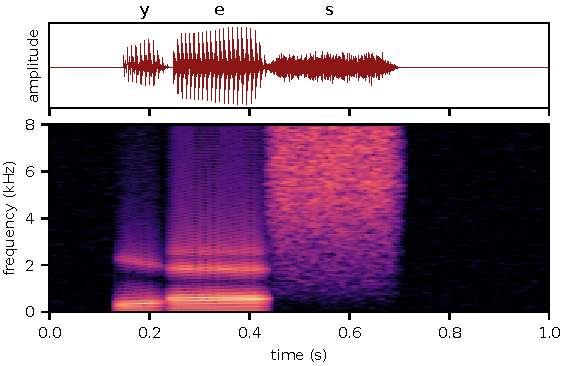
\includegraphics[width=0.66\textwidth]{images/day05/yes_wave_spectrogram.pdf}
  \par\endgroup
  \small
  \begin{itemize}
    \item Top: the samples. You see when the sound is loud. Bottom: the
          spectrogram. Each column is the spectrum of a short piece of the
          signal. A bright point is a strong frequency.
    \item A vowel has horizontal bands at low frequencies. The sound ``s''
          is noise above 4 kHz.
  \end{itemize}
  \source{A synthetic signal with the main properties of the word ``yes''.
    Nobody recorded it.}
\end{frame}

\begin{frame}{Step 1: cut the signal into frames}
  \begingroup\centering
  \begin{tikzpicture}[font=\footnotesize, x=0.2cm, y=1cm]
    % One second: 49 frames of 20 ms.
    \foreach \k in {0,...,48} {
      \draw[coolgray, fill=boxgray] (\k,0) rectangle (\k+1,0.6);
    }
    \draw[cardinalred, line width=1pt, fill=cardinalred!25] (20,0)
      rectangle (21,0.6);
    \node[anchor=west] at (49.5,0.3) {1 s};
    \node[text=coolgray, font=\scriptsize] at (24.5,0.85)
      {16\,000 samples, 49 frames};
    % Zoom on one frame.
    \draw[cardinalred] (20,0) -- (12,-0.6) (21,0) -- (34,-0.6);
    \draw[cardinalred, line width=1pt] (12,-1.5) rectangle (34,-0.6);
    \draw[cardinalred!80!black, line width=0.6pt]
      plot[domain=12.3:33.7, samples=120]
      (\x, {-1.05 + 0.28*sin(90*\x)*cos(17*\x)});
    \node[anchor=west] at (34.5,-1.05) {20 ms, 320 samples};
  \end{tikzpicture}\par\endgroup
  \vskip 0.5em
  \begin{itemize}
    \item A word changes all the time. In 20 to 40 ms, the sound is almost
          constant: the mouth does not move so fast.
    \item \textbf{Frame length:} the duration of one frame, here 20 ms.
    \item \textbf{Frame stride:} the time between the starts of two frames,
          here 20 ms. With a smaller stride, the frames overlap.
    \item Each frame gets one spectrum. The frames in order give the time
          axis of the spectrogram.
  \end{itemize}
  \source{Frame length and stride: kit lab ``KWS Feature Engineering'' of
    \emph{Machine Learning Systems}.}
\end{frame}

\begin{frame}{Step 2: window function and FFT}
  \begingroup\centering
  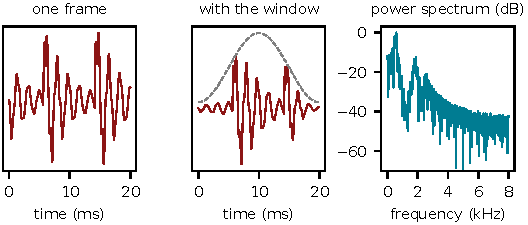
\includegraphics[width=0.82\textwidth]{images/day05/frame_window_fft.pdf}
  \par\endgroup
  \small
  \begin{itemize}
    \item A frame starts and stops suddenly. The FFT sees the two jumps as
          frequencies that are not in the sound. The \textbf{Hamming
          window} makes the two ends of the frame small.
    \item The \textbf{FFT} gives the spectrum of the frame. With 512 points
          at 16 kHz, it has 257 bins with a width of 31.25 Hz, from 0 to
          8 kHz.
    \item The features use the power of each bin: the square of the
          magnitude.
  \end{itemize}
  \source{One frame of the synthetic signal. The FFT adds zeros to the 320
    samples to get 512 points.}
\end{frame}

\begin{frame}{Step 3: the Mel scale}
  \begin{columns}[c]
    \begin{column}{0.50\textwidth}
      \centering
      \begin{tikzpicture}[font=\scriptsize, x=0.46cm, y=1.35cm]
        \draw[->, coolgray] (0,0) -- (8.6,0) node[right] {kHz};
        \draw[->, coolgray] (0,0) -- (0,3.2);
        \node[anchor=west, coolgray] at (0.1,3.15) {Mel};
        \foreach \x in {1,2,4,8} {
          \draw[coolgray] (\x,0) -- (\x,-0.06) node[below] {\x};
        }
        \foreach \y/\l in {1/1000, 2/2000, 2.84/2840} {
          \draw[coolgray] (0,\y) -- (-0.12,\y) node[left] {\l};
        }
        \draw[cardinalred, line width=1pt] plot[domain=0:8, samples=60]
          (\x, {2.595*log10(1 + \x/0.7)});
        \draw[coolgray, dotted] (1,0) -- (1,1) -- (0,1);
        \draw[coolgray, dotted] (8,0) -- (8,2.84) -- (0,2.84);
      \end{tikzpicture}
    \end{column}
    \begin{column}{0.46\textwidth}
      \[
        m = 2595 \cdot \log_{10}\!\left(1 + \frac{f}{700}\right)
      \]
      \small
      \renewcommand{\arraystretch}{1.15}
      \begin{tabular}{@{}rr@{}}
        \toprule
        \textbf{Frequency in Hz} & \textbf{Mel} \\
        \midrule
        500  & 607 \\
        1000 & 1000 \\
        2000 & 1521 \\
        4000 & 2146 \\
        8000 & 2840 \\
        \bottomrule
      \end{tabular}
    \end{column}
  \end{columns}
  \vskip 0.4em
  \begin{itemize}
    \item The ear separates two low tones better than two high tones. The
          Mel scale has equal steps for equal steps of the ear.
    \item The range from 0 to 1 kHz has 1000 Mel. The range from 4 to 8 kHz
          has only 694 Mel.
  \end{itemize}
\end{frame}

\begin{frame}{The Mel filter bank}
  \begingroup\centering
  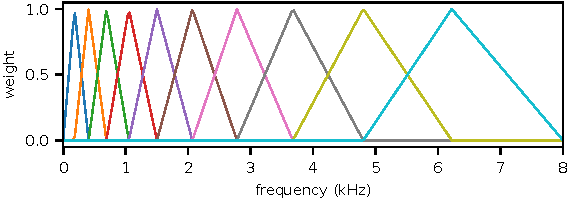
\includegraphics[width=0.86\textwidth]{images/day05/mel_filter_bank.pdf}
  \par\endgroup
  \vskip 0.2em
  \small
  \begin{itemize}
    \item Each triangle is one filter. It adds the power of the bins below
          it, with the weight of the triangle.
    \item The centres of the filters have equal distances on the Mel scale.
          So the filters are narrow at low frequencies and wide at high
          frequencies.
    \item One frame goes from 257 power values to one energy for each
          filter. A typical bank has 20 to 40 filters.
    \item The result for all frames is the \textbf{Mel spectrogram}. Other
          name: Mel filter bank energies (MFE).
  \end{itemize}
  \source{The figure shows 10 filters, so that each filter is visible. The
    example of this part uses 32 filters.}
\end{frame}

\begin{frame}{Step 4: logarithm and DCT}
  \begingroup\centering
  \begin{tikzpicture}[font=\footnotesize, >={Stealth[length=5pt]},
      b/.style={draw=coolgray, rounded corners=3pt, fill=boxgray,
                minimum width=1.9cm, minimum height=0.9cm, align=center},
      lab/.style={font=\scriptsize, text=coolgray, align=center}]
    \node[b] (a) at (0,0)   {32 Mel\\energies};
    \node[b] (b) at (2.9,0) {Logarithm};
    \node[b] (c) at (5.8,0) {DCT};
    \node[b, draw=cardinalred] (d) at (8.7,0) {13\\coefficients};
    \foreach \a/\b in {a/b, b/c, c/d} { \draw[->] (\a) -- (\b); }
    \node[lab] at (4.35,-0.85) {for each frame};
  \end{tikzpicture}\par\endgroup
  \vskip 0.4em
  \begin{itemize}
    \item \textbf{Logarithm.} The ear hears loudness on a logarithmic
          scale. The logarithm also makes a loud voice and a quiet voice
          more equal.
    \item \textbf{Discrete cosine transform (DCT).} The energies of
          neighbour filters are almost equal. The DCT writes the 32 values
          as a sum of cosine curves.
    \item The first coefficients give the smooth form of the spectrum. This
          form separates the speech sounds. The last coefficients give the
          fine detail.
    \item Keep the first 12 or 13 coefficients. These are the
          \textbf{Mel-frequency cepstral coefficients (MFCC)}.
  \end{itemize}
  \source{Steps and typical values: kit lab ``KWS Feature Engineering'' of
    \emph{Machine Learning Systems}.}
\end{frame}

\begin{frame}{From 16\,000 samples to 637 values}
  \begingroup\centering
  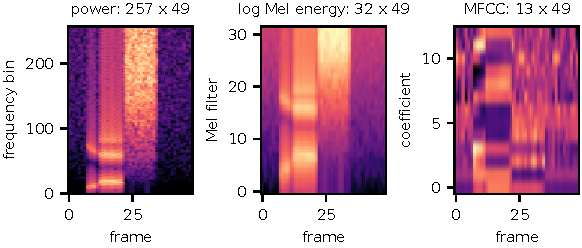
\includegraphics[width=0.74\textwidth]{images/day05/mfcc_steps.pdf}
  \par\endgroup
  \begin{columns}[c]
    \begin{column}{0.68\textwidth}
      \footnotesize
      \renewcommand{\arraystretch}{1.05}
      \begin{tabular}{@{}L{0.27\textwidth}L{0.50\textwidth}r@{}}
        \toprule
        \textbf{After the step} & \textbf{Size} & \textbf{Values} \\
        \midrule
        Samples of 1 s  & 16\,000              & 16\,000 \\
        Frames and FFT  & 49 frames of 257 bins & 12\,593 \\
        Mel filter bank & 49 frames of 32 energies & 1568 \\
        DCT             & 49 frames of 13 coefficients & \textbf{637} \\
        \bottomrule
      \end{tabular}
    \end{column}
    \begin{column}{0.28\textwidth}
      \small
      The model gets 25 times fewer values than the microphone gives.
    \end{column}
  \end{columns}
  \source{The steps for the synthetic word ``yes''. The picture of the MFCC
    scales each coefficient alone, so that all rows are visible.}
\end{frame}

\begin{frame}{Spectrogram, Mel energies, or MFCC}
  \small
  \renewcommand{\arraystretch}{1.3}
  \begin{tabular}{@{}L{0.20\textwidth}L{0.22\textwidth}L{0.22\textwidth}L{0.24\textwidth}@{}}
    \toprule
    & \textbf{Spectrogram} & \textbf{Mel energies (MFE)} & \textbf{MFCC} \\
    \midrule
    Steps       & Frames, FFT & and the Mel filters, the logarithm
                & and the DCT \\
    Values for 1 s & Most & Fewer & Fewest \\
    Keeps       & All detail of the frequencies
                & The detail that the ear hears
                & The smooth form of the spectrum \\
    Good for    & Machines, music, sounds of animals
                & Sounds of the environment
                & Speech: keywords, speakers \\
    \bottomrule
  \end{tabular}
  \vskip 0.6em
  \begin{itemize}
    \item Edge Impulse Studio gives the three as processing blocks. You
          select one in the lab.
    \item The feature block is a design decision. Train the model with two
          blocks, and compare the accuracy and the time on the device.
  \end{itemize}
  \source{Comparison: kit lab ``KWS Feature Engineering'' of \emph{Machine
    Learning Systems}.}
\end{frame}

% ------------------------------------------------------------------ the model
\begin{frame}{The model: a small CNN on the MFCC image}
  \small
  \renewcommand{\arraystretch}{1.2}
  \begin{tabular}{@{}L{0.46\textwidth}L{0.22\textwidth}r@{}}
    \toprule
    \textbf{Layer} & \textbf{Output} & \textbf{Parameters} \\
    \midrule
    Input: 49 frames of 13 coefficients & $49 \times 13$ & none \\
    Convolution, 8 filters of 3 frames, ReLU & $49 \times 8$ & 320 \\
    Max pooling, 2 frames     & $25 \times 8$ & none \\
    Convolution, 16 filters of 3 frames, ReLU & $25 \times 16$ & 400 \\
    Max pooling, 2 frames     & $13 \times 16$ & none \\
    Fully connected, softmax  & 4 & 836 \\
    \midrule
    Total & & \textbf{1556} \\
    \bottomrule
  \end{tabular}
  \vskip 0.5em
  \begin{itemize}
    \item The convolutions go along the time axis. The 13 coefficients of a
          frame are the channels of the first layer.
    \item In \code{int8}, the weights need about 1.6 KB of flash.
  \end{itemize}
  \source{The model of the kit lab ``Keyword Spotting (KWS)''. Parameter
    counts: the training notebook of the repository XIAO-ESP32S3-Sense.}
\end{frame}

\begin{frame}{Why a convolution along the time axis}
  \begin{columns}[c]
    \begin{column}{0.46\textwidth}
      \centering
      \begin{tikzpicture}[font=\scriptsize, x=0.19cm, y=0.22cm]
        % The MFCC image: 22 frames shown, 7 rows shown.
        \foreach \k in {0,...,21} {
          \foreach \r in {0,...,6} {
            \draw[coolgray!50, fill=boxgray] (\k,\r) rectangle (\k+1,\r+1);
          }
        }
        \fill[cardinalred!45] (5,0) rectangle (11,7);
        \fill[darkcyan!30] (12,0) rectangle (18,7);
        \draw[cardinalred, line width=1.1pt] (7,0) rectangle (10,7);
        \draw[->, cardinalred, line width=0.8pt] (10.4,3.5) -- (13.5,3.5);
        \node[below] at (11,-0.3) {time: frames};
        \node[rotate=90, above] at (-0.3,3.5) {coefficients};
        \node[cardinalred, above] at (8.5,7.1) {filter of 3 frames};
      \end{tikzpicture}
    \end{column}
    \begin{column}{0.52\textwidth}
      \small
      \begin{itemize}
        \item A keyword can start at any time in the window.
        \item A filter looks at 3 frames: 60 ms. It moves along the window
              with the same weights.
        \item So the filter finds a sound at each position. A fully
              connected layer must learn each position alone.
        \item The pooling layers make the result less sensitive to a small
              shift.
      \end{itemize}
    \end{column}
  \end{columns}
  \vskip 0.5em
  \begin{itemize}
    \item Larger keyword models use depthwise separable convolutions on
          the image of time and frequency. Day 6 explains this layer.
  \end{itemize}
  \source{Model types for keyword spotting: Zhang et al., ``Hello Edge:
    Keyword Spotting on Microcontrollers'', 2017.}
\end{frame}

\begin{frame}{Four classes: two keywords, unknown, and noise}
  \begin{columns}[T]
    \begin{column}{0.46\textwidth}
      \small
      \renewcommand{\arraystretch}{1.3}
      \begin{tabular}{@{}L{0.34\textwidth}L{0.58\textwidth}@{}}
        \toprule
        \textbf{Class} & \textbf{Content} \\
        \midrule
        YES     & The first keyword \\
        NO      & The second keyword \\
        UNKNOWN & Other words \\
        NOISE   & No speech: the room, a fan, a street \\
        \bottomrule
      \end{tabular}
    \end{column}
    \begin{column}{0.50\textwidth}
      \begin{itemize}
        \item A softmax always gives probabilities with the sum 1.
        \item With two classes only, each sound is ``yes'' or ``no'': a
              door, a cough, the word ``yesterday''.
        \item The two other classes give the model a correct answer for a
              sound that is not a keyword.
      \end{itemize}
    \end{column}
  \end{columns}
  \vskip 0.5em
  \begin{itemize}
    \item The device hears a keyword only some seconds each day. Almost all
          windows are noise or other words.
  \end{itemize}
  \keypoint{The classes UNKNOWN and NOISE are the classes that the device
    sees most of the time. Their quality decides the false activations.}
  \source{Classes: kit lab ``Keyword Spotting (KWS)'' of \emph{Machine
    Learning Systems}.}
\end{frame}

\begin{frame}{The dataset for a keyword model}
  \begin{columns}[T]
    \begin{column}{0.49\textwidth}
      \begin{block}{A public dataset}
        \begin{itemize}
          \item Speech Commands: 35 words, more than 1000 clips of each
                word, 1 s for each clip, many speakers.
          \item It gives the keywords and the class UNKNOWN.
        \end{itemize}
      \end{block}
    \end{column}
    \begin{column}{0.47\textwidth}
      \begin{block}{Your recordings}
        \begin{itemize}
          \item The keywords with your voice and your microphone.
          \item The noise of your room.
          \item Cut each recording into clips of 1 s.
        \end{itemize}
      \end{block}
    \end{column}
  \end{columns}
  \vskip 0.4em
  \begin{itemize}
    \item The rules of Day 2 apply: all speakers of the test set are new
          speakers, and each class has a similar number of clips.
    \item Data augmentation makes more clips from one clip: add noise, move
          the word in the window, hide some frames or some coefficients.
  \end{itemize}
  \source{Dataset: Warden, ``Speech Commands: A Dataset for
    Limited-Vocabulary Speech Recognition'', 2018; kit lab ``Keyword
    Spotting (KWS)''.}
\end{frame}

% ------------------------------------------------------------------ the errors
\begin{frame}{Two errors: false accept and false reject}
  \begin{columns}[c]
    \begin{column}{0.52\textwidth}
      \small
      \renewcommand{\arraystretch}{1.4}
      \setlength{\tabcolsep}{4pt}
      \begin{tabular}{@{}L{0.32\textwidth}L{0.27\textwidth}L{0.27\textwidth}@{}}
        \toprule
        & \textbf{Device says keyword} & \textbf{Device says nothing} \\
        \midrule
        \textbf{Keyword spoken} & Correct & \textcolor{cardinalred}{False
                                            reject} \\
        \textbf{No keyword}     & \textcolor{cardinalred}{False accept}
                                & Correct \\
        \bottomrule
      \end{tabular}
    \end{column}
    \begin{column}{0.45\textwidth}
      \begin{itemize}
        \item \textbf{False reject rate (FRR):} the part of the spoken
              keywords that the device misses.
        \item \textbf{False accept rate (FAR):} the part of the other
              windows that start the device.
      \end{itemize}
    \end{column}
  \end{columns}
  \vskip 0.5em
  \begin{itemize}
    \item The user feels the two errors in different ways. A false reject:
          ``I must say it again.'' A false accept: ``It starts alone.''
    \item One accuracy number mixes the two errors. For a keyword spotter,
          report the two rates.
  \end{itemize}
  \keypoint{For an always-on device, report the false accepts for each
    hour, and the false reject rate.}
  \source{Metrics: \emph{Machine Learning Systems}, Volume I, chapter 4.}
\end{frame}

\begin{frame}{The threshold moves the two errors}
  \begingroup\centering
  \begin{tikzpicture}[font=\scriptsize, x=1.6cm, y=1.5cm]
    \draw[->, coolgray] (0,0) -- (5.4,0)
      node[right, align=left] {probability\\of ``yes''};
    \node[below, coolgray] at (0,0) {0};
    \node[below, coolgray] at (5,0) {1};
    \fill[darkcyan!25] plot[domain=3.2:5, samples=30]
      (\x, {1.1*exp(-(\x-1.4)*(\x-1.4)/1.1)}) -- (5,0) -- (3.2,0) -- cycle;
    \fill[cardinalred!25] plot[domain=0.6:3.2, samples=40]
      (\x, {1.2*exp(-(\x-4.0)*(\x-4.0)/0.7)}) -- (3.2,0) -- (0.6,0) -- cycle;
    \draw[darkcyan, line width=0.9pt] plot[domain=0:5, samples=60]
      (\x, {1.1*exp(-(\x-1.4)*(\x-1.4)/1.1)});
    \draw[cardinalred, line width=0.9pt] plot[domain=0:5, samples=60]
      (\x, {1.2*exp(-(\x-4.0)*(\x-4.0)/0.7)});
    \draw[line width=0.9pt, dashed] (3.2,0) -- (3.2,1.45)
      node[above] {threshold};
    \node[darkcyan] at (1.2,1.25) {windows with no keyword};
    \node[cardinalred] at (4.45,1.35) {keyword};
    \node[darkcyan, align=center] at (3.75,-0.35) {false accepts};
    \node[cardinalred, align=center] at (2.55,-0.35) {false rejects};
  \end{tikzpicture}\par\endgroup
  \vskip 0.3em
  \begin{itemize}
    \item The device accepts a keyword when its probability is above a
          threshold.
    \item A higher threshold gives fewer false accepts and more false
          rejects. A lower threshold does the opposite.
    \item The model fixes the two curves. The threshold selects the point
          on the trade-off. You can change it after the training.
  \end{itemize}
  \source{The curves are an example. They are not a measurement.}
\end{frame}

\begin{frame}{An always-on device makes many decisions}
  \small
  \renewcommand{\arraystretch}{1.1}
  \begin{tabular}{@{}L{0.62\textwidth}r@{}}
    \toprule
    \textbf{Quantity} & \textbf{Value} \\
    \midrule
    New window                               & each 0.5 s \\
    Inferences in one hour                   & 7200 \\
    Inferences in one day                    & 172\,800 \\
    \midrule
    False accept rate of 0.1 percent: false accepts in one hour & 7.2 \\
    The same rate: false accepts in one day  & 173 \\
    Rate for one false accept in one day     & 0.0006 percent \\
    \bottomrule
  \end{tabular}
  \vskip 0.2em
  \begin{itemize}
    \item A model with 99.9 percent of correct windows starts the device 7
          times each hour with no reason.
    \item The model alone cannot reach 0.0006 percent. The post-processing
          of Part 3 uses more than one window for one decision.
  \end{itemize}
  \keypoint{A very small error rate for each window becomes a large number
    of errors, because the device never stops.}
  \source{The values are a calculation for one window each 0.5 s.}
\end{frame}

\begin{frame}{The cost on the device}
  \begin{columns}[T]
    \begin{column}{0.49\textwidth}
      \begin{block}{The features}
        \begin{itemize}
          \item 49 FFTs, the filter bank, and the DCT for each window.
          \item The Studio estimates 675 ms and 16 KB of RAM for the MFCC
                block of the kit lab, on a board with an ESP32.
        \end{itemize}
      \end{block}
    \end{column}
    \begin{column}{0.47\textwidth}
      \begin{block}{The model}
        \begin{itemize}
          \item 1556 parameters.
          \item In \code{int8}, the largest sum of an input and an output
                is $637 + 392 = 1029$ bytes.
        \end{itemize}
      \end{block}
    \end{column}
  \end{columns}
  \vskip 0.4em
  \begin{itemize}
    \item The features can need more time than the model. This is the
          result of Day 3 for motion data also.
    \item To make the device faster, change the features first: a shorter
          FFT, fewer coefficients, a larger frame stride.
    \item In the lab you read the two times from the Serial Monitor: the
          time for the features (DSP) and the time for the classification.
  \end{itemize}
  \source{Estimates of Edge Impulse Studio for the ESP-EYE: kit lab
    ``Keyword Spotting (KWS)''. Nobody measured the times on the kit of this
    course.}
\end{frame}

% -------------------------------------------------------------------- exercise
\exerciseframe{match spectrograms to words}{%
  \small
  The three spectrograms show the words ``yes'', ``no'', and ``six''. Each
  picture has 1 s.
  \vskip 0.2em
  \begingroup\centering
  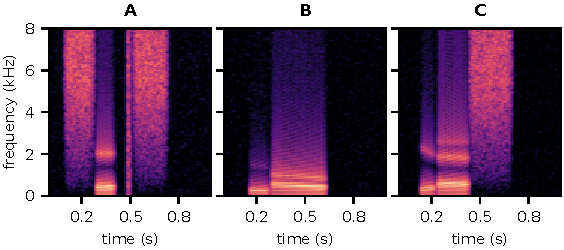
\includegraphics[width=0.74\textwidth]{images/day05/exercise_spectrograms.pdf}
  \par\endgroup
  \vskip 0.2em
  \begin{enumerate}
    \item Which word is A, which is B, and which is C? Give one reason for
          each picture.
    \item Which two words are most difficult to separate for a model? Why?
    \item A model sees only the frequencies below 2 kHz. Which two words
          can it still separate?
  \end{enumerate}
  Work with your neighbour for 8 minutes. The signals are synthetic.
}

\answerframe{match spectrograms to words}{%
  \small
  \begin{enumerate}
    \item \textbf{A is ``six''.} It has noise above 4 kHz at the start and
          at the end: the two sounds ``s''. Between them is a short vowel,
          then a pause, and a short burst: the sound ``k''.

          \textbf{B is ``no''.} It has no noise at high frequencies. All
          its power is in bands below 1.5 kHz: the sound ``n'' and a
          vowel.

          \textbf{C is ``yes''.} It starts with bands at low frequencies,
          and one band moves down: the sounds ``y'' and ``e''. It ends
          with noise above 4 kHz: the sound ``s''.
    \item ``yes'' and ``six''. The two words have a vowel and then the
          sound ``s''. Only the start is different.
    \item ``no'' against the two other words: the vowel of ``no'' has its
          bands below 1 kHz, and the vowels of ``yes'' and ``six'' have a
          band near 2 kHz. Below 2 kHz, the sound ``s'' has almost no
          power, so ``yes'' and ``six'' look more equal.
  \end{enumerate}
  \vskip 0.2em
  A model does this work with the MFCC image. It looks for the same
  patterns: where is the power, and when does it change.
}

% Part 2 of Day 5: Vision under microcontroller constraints.
%
% Topics of the syllabus: input resolution, width multiplier, visual wake
% words; peak activation memory and PSRAM; transfer learning; capture, resize,
% and colour conversion on the device. Exercise: calculate the peak activation
% memory of a MobileNet at two input resolutions.

\theorypart{Vision under microcontroller constraints}%
  {calculate the peak activation memory of a MobileNet at two resolutions}

% Part 3 of Day 5: Streaming inference and detection.
%
% Topics of the syllabus: sliding windows, smoothing, thresholds; cascade: an
% always-on microcontroller wakes a larger device; why SSD and YOLO do not fit
% on a microcontroller; the centroid method of FOMO. Exercise: design the
% cascade for a voice-controlled camera.

\theorypart{Streaming inference and detection}%
  {design the cascade for a voice-controlled camera}

% Recap of the day. Three to five points, then the one point to keep.
\begin{frame}{Recap}
  \begin{itemize}
    \item An audio model does not take samples. It takes a small image of the
          sound: MFCC features of short frames.
    \item A keyword spotting model needs a class for unknown words and a class
          for noise. You tune it with the false accept rate and the false
          reject rate.
    \item For a vision model, the peak activation memory decides if the model
          fits. A smaller image and a narrower network decrease it.
    \item A stream gives many results each second. Smoothing and a threshold
          turn them into one decision. A cascade keeps the large device
          asleep.
  \end{itemize}
  \vskip 0.5em
  \keypoint{On a microcontroller, the model is one part of a pipeline. The
            features before the model and the post-processing after the model
            decide the result as much as the model.}
\end{frame}

% Further reading. The list comes from the "Sources" part of Day 5 in the
% syllabus.
\begin{frame}{Further reading}
  \footnotesize
  \begin{block}{Book chapters}
    \begin{itemize}
      \item \emph{Machine Learning Systems} (mlsysbook.ai), Volume I: chapter
            6 ``Network Architectures'', section ``CNNs: Spatial Pattern
            Processing''.
      \item \emph{Machine Learning Systems}, XIAOML Kit labs: ``Keyword
            Spotting (KWS)'', ``KWS Feature Engineering'', and ``Image
            Classification''.
    \end{itemize}
  \end{block}
  \begin{block}{Papers}
    \begin{itemize}
      \item ``Hello Edge: Keyword Spotting on Microcontrollers'', Zhang et
            al., 2017.
      \item ``Speech Commands: A Dataset for Limited-Vocabulary Speech
            Recognition'', Warden, 2018.
      \item ``Visual Wake Words Dataset'', Chowdhery et al., 2019.
      \item ``MCUNet: Tiny Deep Learning on IoT Devices'', Lin et al., 2020.
    \end{itemize}
  \end{block}
  \begin{block}{Tools}
    \begin{itemize}
      \item Edge Impulse documentation, with the pages on MFCC and on FOMO:
            \url{https://docs.edgeimpulse.com}
    \end{itemize}
  \end{block}
\end{frame}

% Credits frame. Section 10 of the syllabus gives this text.
% Each deck ends with this frame:
%   % Credits frame. Section 10 of the syllabus gives this text.
% Each deck ends with this frame:
%   % Credits frame. Section 10 of the syllabus gives this text.
% Each deck ends with this frame:
%   \input{sections/credits}
%
% The list \coursecredits selects the sources. preamble/course.tex gives the
% default list and one command for each source. The main file of a deck
% changes the list before it inputs this file, so that the frame names only
% the sources that the deck uses:
%   \renewcommand{\coursecredits}{\creditmlsys\creditxiao}
\begin{frame}[allowframebreaks]{Credits}
  \vskip 0.6em
  \begin{itemize}\footnotesize\itemsep 0.4em
    \coursecredits
  \end{itemize}
  \vskip 0.8em
\end{frame}

%
% The list \coursecredits selects the sources. preamble/course.tex gives the
% default list and one command for each source. The main file of a deck
% changes the list before it inputs this file, so that the frame names only
% the sources that the deck uses:
%   \renewcommand{\coursecredits}{\creditmlsys\creditxiao}
\begin{frame}[allowframebreaks]{Credits}
  \vskip 0.6em
  \begin{itemize}\footnotesize\itemsep 0.4em
    \coursecredits
  \end{itemize}
  \vskip 0.8em
\end{frame}

%
% The list \coursecredits selects the sources. preamble/course.tex gives the
% default list and one command for each source. The main file of a deck
% changes the list before it inputs this file, so that the frame names only
% the sources that the deck uses:
%   \renewcommand{\coursecredits}{\creditmlsys\creditxiao}
\begin{frame}[allowframebreaks]{Credits}
  \vskip 0.6em
  \begin{itemize}\footnotesize\itemsep 0.4em
    \coursecredits
  \end{itemize}
  \vskip 0.8em
\end{frame}


\end{document}
